% ====================================================================
\section{Results and analysis}\label{sec:results}
% ====================================================================
All numbers in this report come from the analysis script \texttt{analysis/analysis.py} in the repository linked on the
title page, which also contains the raw data. Uncertainties are standard deviations ($1\sigma$). I fitted all lines by
nonlinear least squares with a linear baseline; \cref{app:errors} explains the uncertainties.

% --------------------------------------------------------------------
\subsection{Frequency and reference field}\label{sec:frequency}
During the DPPH measurements the frequency counter showed on average $\nu=\qty{9.359378}{GHz}$ (twelve readings, scatter
\qty{22}{kHz}), so the frequency is known far better than any field. For \ce{MnCl2} it was $\nu=\qty{9.352713}{GHz}$.
With the literature value $g_\text{DPPH}=\num{2.0036(2)}$~\cite{poole1996}, \cref{eq:resonance} puts the DPPH resonance at
\begin{equation}\label{eq:bdpph}
  B_\text{DPPH}=\qty{333.75(3)}{mT}.
\end{equation}

% --------------------------------------------------------------------
\subsection{Magnetic field: hysteresis and calibration}\label{sec:field}

\begin{figure}[t]
  \centering
  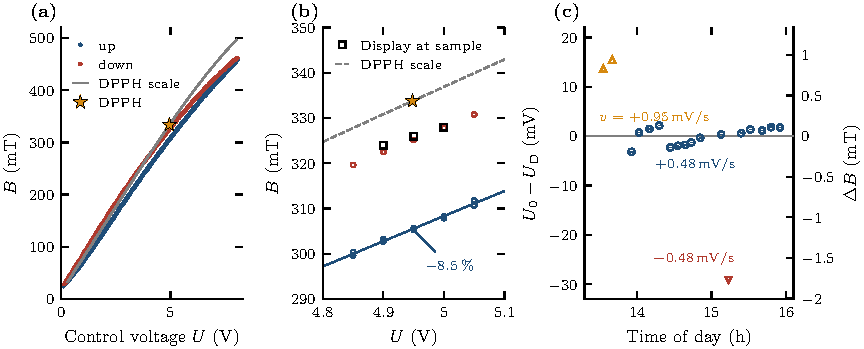
\includegraphics[width=\textwidth]{figures/field.pdf}
  \caption{Main field. (a)~Hall probe (analog output) over the full range: upward (01, 03) and downward (02); in gray the
  field scale calibrated with DPPH (\cref{eq:fieldscale}). (b)~Close-up around the DPPH line: analog output, display at the
  sample position (measurement 19) and the DPPH field (star). The analog output lies \qty{8.5}{\percent}, the display
  \qty{2.3}{\percent} below the DPPH field. (c)~Position $U_0$ of the DPPH line in all scans relative to the mean
  $U_\text{D}$ of the eleven reference scans; triangles: earlier start and doubled sweep rate (orange), down-sweep (red).}
  \label{fig:field}
\end{figure}

\paragraph{Hysteresis.}
Without a sample, I swept the field over the full range up (01, 03) and down (02) (\cref{fig:field}a). Between
\qty{1}{V} and \qty{5.5}{V} the down-sweep lies \qtyrange{14}{24}{mT} above the up-sweeps, and at \qty{0}{V} a residual
field of \qtyrange{17}{24}{mT} remains. I attribute this to hysteresis of the iron yoke: the power supply sets the coil current
via $U$, but the field in the gap also depends on how the iron was magnetized before. For the calibration I use
only up-sweeps, which all start at \qty{0}{V}. Above \qty{0.3}{V} both are described by a cubic polynomial
$B_\text{Hall}(U)$ (scatter \qty{1.1}{mT}).

\paragraph{Calibration.}
In the eleven reference scans (09 to 15 and 24 to 27: jump from \qty{0}{V} to \qtyrange{4.895}{4.910}{V}, wait
\qty{60}{s}, then \qty{0.48}{mV/s}) the DPPH line, more precisely its position $U_0$ in \cref{eq:convolution}, lies on average
at $U_\text{D}=\qty{4.9480}{V}$ (scatter \qty{1.9}{mV}). There the analog output reads \qty{305.4}{mT}, and the display,
read with the probe tip at the center of the cavity, \qty{326}{mT} (\cref{fig:field}b). As $g$-factors these would be
\num{2.189} and \num{2.052} instead of \num{2.0036}. The Hall probe reads too low, the analog output by
\qty{8.5}{\percent} and the display by \qty{2.3}{\percent}.

These are two separate effects. Over the whole range the analog output lies about \qty{6}{\percent} below the display of
the same probe. The probe position would change both readings equally, so the analog output has a scale error of its
own. The remaining \qty{2.3}{\percent} of the display may come from the probe position. According to the course
supervisor (private communication), the gaussmeter is new and may be slightly miscalibrated, and a reading that is too
low usually means that the sensor is not at the height and orientation of maximum reading. A tilt of only \ang{12}
would already explain \qty{2.3}{\percent} ($\cos\ang{12}=\num{0.978}$). The data cannot tell whether the probe sat at its
maximum. I therefore use the gaussmeter only for the \emph{shape} of $B(U)$ and take the scale from DPPH:
\begin{equation}\label{eq:fieldscale}
  B(U)=k\,B_\text{Hall}(U),\qquad k=\frac{B_\text{DPPH}}{B_\text{Hall}(U_\text{D})}=\num{1.0927},
  \qquad \frac{\dd B}{\dd U}\Big|_{U_\text{D}}=\qty{60.76}{mT/V}.
\end{equation}
With this calibration $g_\text{DPPH}$ is no longer measured but sets the scale. I determine the $g$-factor of \ce{MnCl2}
relative to DPPH, so the scale error of the probe cancels. Widths are converted from volts to millitesla with the slope
$\dd B/\dd U$.

\paragraph{The field lags behind.}
With the same protocol the line position is very reproducible. In the eleven scans starting at \qty{4.910}{V} it scatters
by only \qty{0.27}{mV} once a slow drift is removed (\cref{fig:field}c). When the protocol changes, the line jumps. If
the scan starts \qty{75}{mV} earlier (07b, 08), the line lies \qty{19}{mV} higher; in down-sweep~18 it lies \qty{29}{mV}
lower. Ordinary hysteresis cannot explain the first jump, because these scans also start at \qty{0}{V} and run on the
same rising branch. The field lags behind the set value, probably because of a magnetic after-effect in the iron yoke:
it catches up during the wait and falls behind again once the sweep continues. The lag is \qty{22(3)}{\percent} of the
distance swept since the wait and stops growing after a few hundred millivolts (\cref{sec:mncl2}).

This has two consequences. The calibration \cref{eq:fieldscale} only holds for scans run the same way, so the \ce{MnCl2}
scan needs its own reference (\cref{sec:mncl2}). And during the slow scans the field probably rises more slowly than the
static slope says. Since I convert widths with the static slope, they could be up to \qty{22}{\percent} too large. I treat
this as a one-sided systematic.

% --------------------------------------------------------------------
\subsection{DPPH: line width and \texorpdfstring{$T_2$}{T2}}\label{sec:dpph}

\begin{figure}[t]
  \centering
  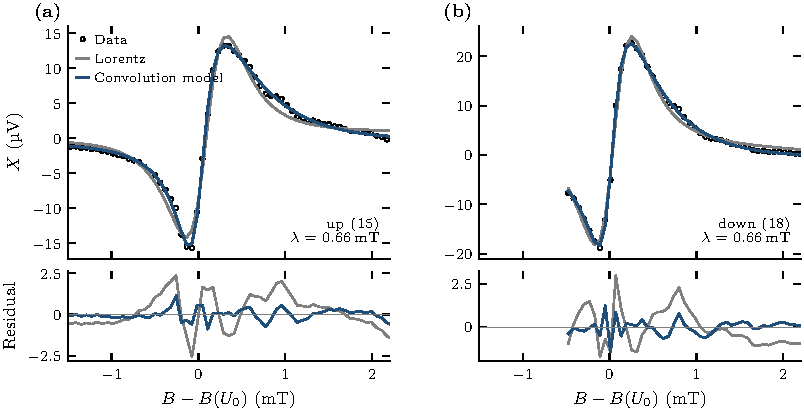
\includegraphics[width=\textwidth]{figures/lineshape.pdf}
  \caption{DPPH line in up-sweep 15 and in down-sweep 18 (otherwise identical settings), shown as the signal $S=-X$
  (\cref{sec:setup}): the derivative of the absorption is positive on the rising and negative on the falling side. Gray: Lorentzian line; blue:
  Lorentzian line convolved with a one-sided field distribution of length $\lambda$ (\cref{eq:convolution}). Bottom: the
  residuals (measurement minus fit). The long tail lies on the high-field side in both sweep directions.}
  \label{fig:lineshape}
\end{figure}

\paragraph{Line shape.}
All DPPH scans show the derivative absorption line from \cref{sec:modulation}, but slightly asymmetric: the flank toward
high field is flatter and longer (\cref{fig:lineshape}). A Lorentzian fits the center but leaves systematic residuals,
and a Gaussian is worse (1.8 times larger residuals). I suspect that the asymmetry comes from field inhomogeneity
across the relatively large powder sample. Parts of the sample would then reach resonance at slightly higher coil
currents, which gives a tail toward high field. To account for this, I fitted a Lorentzian convolved with a one-sided
exponential field distribution of length $\lambda$:
\begin{equation}\label{eq:convolution}
  S(U)=\int_0^\infty\frac{\dd u}{\lambda}\,e^{-u/\lambda}\,
  \frac{\dd}{\dd x}\biggl[\frac{a}{1+x^2}+\frac{d\,x}{1+x^2}\biggr]_{x=(U-U_0-u)/G}+b_0+b_1U .
\end{equation}
Here $U_0$ is the line position without the tail and $G$ the HWHM of the Lorentzian in units of the control voltage. The
amplitudes $a$ and $d$ belong to absorption and dispersion; a small dispersion part is needed because the bridge phase is
never exactly zero. The baseline is $b_0+b_1U$. This model reduces the residuals by a factor of 3. The length
$\lambda=\qty{13.5(5)}{mV}$ corresponds to \qty{0.82}{mT}, or \qty{0.25}{\percent} of the field. Down-sweep~18 supports
this explanation over the field lag: a lag would move the tail to the other side when sweeping down, but the tail stays
on the same side with the same length. \Cref{tab:dpphfits} in \cref{app:fits} lists the fit results
of every DPPH scan.

\paragraph{Width and \texorpdfstring{$T_2$}{T2}.}
The data do not show what the field distribution looks like at its edge. Other distributions (gamma, half-Cauchy) fit
just as well but give a $G$ up to \qty{10}{\percent} smaller. I take the middle of this range, $G=\qty{3.43}{mV}$, and
with \cref{eq:t2} and the slope from \cref{eq:fieldscale} obtain
\begin{equation}\label{eq:t2dpph}
  \Bpp=\frac{2}{\sqrt3}\,G\,\frac{\dd B}{\dd U}=\qty{0.240(15)}{mT},\qquad
  T_2=\frac{2}{\sqrt3\,\gamma\,\Bpp}=\qty{27(2)}{ns}.
\end{equation}
Most of the uncertainty comes from this choice of model (half the range, \qty{0.013}{mT}); field scale
(\qty{0.007}{mT}) and statistics (\qty{0.003}{mT}) contribute less. If the field rises more slowly during the scan than
assumed (\cref{sec:field}), the line is up to \qty{22}{\percent} narrower and $T_2$ up to \qty{35}{ns} long. A bound
without any model also exists. The simple Lorentzian fit assigns the whole field distribution to the line and gives
$\Bpp=\qty{0.51}{mT}$. Since the distribution can only broaden the line, $T_2\geq\qty{12.8}{ns}$. Reported values for
DPPH are \qtyrange{0.15}{0.47}{mT}~\cite{poole1996}, depending on crystal form and included solvent; my value lies in
this range.

This measurement cannot give the $g$-factor of DPPH independently, because DPPH is the calibration. With the display of
the Hall probe alone I would have obtained $g=\num{2.052}$, \qty{2.4}{\percent} above the literature value. This matches
the \qty{2.3}{\percent} by which the display reads too low.

% --------------------------------------------------------------------
\subsection{Modulation amplitude}\label{sec:modamp}

\begin{figure}[t]
  \centering
  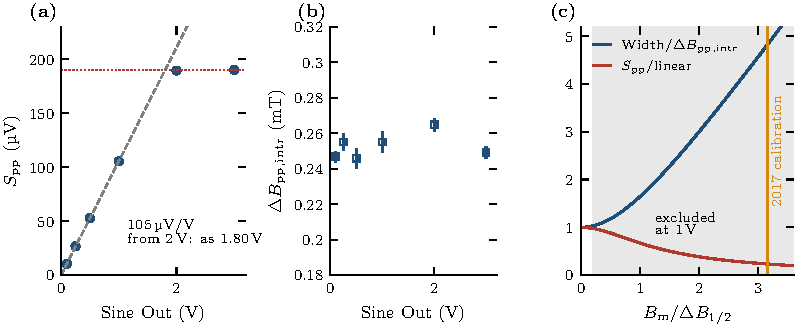
\includegraphics[width=\textwidth]{figures/modulation.pdf}
  \caption{Modulation series (scans 07b to 12). (a)~Peak-to-peak signal versus the Sine Out voltage: proportional up to
  \qty{1}{V}; from \qty{2}{V} on, the amplifier limits. (b)~Width of the Lorentzian line in the convolution model:
  independent of the modulation. (c)~Calculated width and amplitude of the first harmonic of a pure Lorentzian line versus
  $\Bm/\Bhalf$. Gray: excluded at \qty{1}{V} for a pure Lorentzian line (for the measured profile the limit lies slightly
  higher, \cref{eq:bm}); orange: what the 2017 calibration would give at \qty{1}{V}.}
  \label{fig:modulation}
\end{figure}

I tried to measure the alternating field of the modulation coils directly with the gaussmeter in AC mode, at the
modulation frequency of \qty{133}{Hz} and on its most sensitive range, \qty{30}{mT} (\qty{300}{G}, resolution
\qty{10}{\micro T}). The F.\,W.\,Bell 5080 has no lower range, and its bandwidth (dc to \qty{20}{kHz}) covers
\qty{133}{Hz}~\cite{fwbell}. At all Sine Out voltages (\qtyrange{0.1}{4}{V}) it showed only its noise
(\qty{0.04}{mT}). The limit was therefore the sensitivity, not the frequency: the bound derived below,
$\Bm<\qty{0.06}{mT}$ at \qty{1}{V} and $<\qty{0.11}{mT}$ in the limited state, is comparable to this noise. A very
low modulation frequency (e.g.\ \qty{0.1}{Hz}) would have let me follow the oscillating field in DC mode and average
over many periods; I did not try this. Such a calibration would still have to be transferred to \qty{133}{Hz}, because
the inductive impedance of the modulation coils grows with frequency. Since the direct measurement failed, the DPPH
lines themselves give an upper bound on $\Bm$.

In the modulation series I changed only the Sine Out voltage $U_\mathrm m$ (\cref{fig:modulation}). Up to \qty{1}{V} the
peak-to-peak signal $S_\mathrm{pp}$ (the distance between maximum and minimum of the line) grows in proportion to
$U_\mathrm m$ (\qty{105.4}{\micro V/V}, scatter about \qty{1}{\percent}), as \cref{eq:harmonic} requires for small
$\Bm$. At \qty{2}{V} and \qty{3}{V} the signal is the same, \qty{190}{\micro V}: the modulation amplifier limits, and
both settings act like \qty{1.80}{V}. The width does not change; the ratio of the widths in the limited state and at
\qtyrange{0.1}{1}{V} is \num{1.025(36)}.

This is what bounds $\Bm$. In the limited state the signal, and with it $\Bm$, is 1.8 times as large as at \qty{1}{V},
yet the line is not wider. \Cref{fig:modulation}c shows how a line broadens as $\Bm$ grows. For the width ratio to stay
below its upper $2\sigma$ limit of \num{1.096}, the measured line profile requires
\begin{equation}\label{eq:bm}
  \Bm(\qty{1}{V})<\qty{0.059}{mT},\qquad \Bm(\text{limited})<\qty{0.11}{mT}.
\end{equation}
At \qty{1}{V}, the setting of all other DPPH scans, $\Bm$ is at most a quarter of $\Bpp$ and broadens the
fitted line by at most \qty{3}{\percent}. A previous report on this setup gives the 2017 calibration
$\Bm=\qty{5.06}{G/V}\cdot U_\mathrm m+\qty{1.8}{G}$. At \qty{1}{V} this would be \qty{0.69}{mT}, almost three times
$\Bpp$. The line would then be 2.8 times wider at \qty{1}{V} than at \qty{0.1}{V}, and the signal would grow by only a
factor of 1.1 in between. I measured equal widths (ratio \num{1.03(3)}) and a factor of 10.1, so the old calibration does
not hold for the present setup.

\paragraph{Effect of the modulation amplitude.}
As long as $\Bm$ is small compared with the line width, the signal grows in proportion to $\Bm$ and the line shape stays
the same. A large $\Bm$ gives a good signal-to-noise ratio, a small one an undistorted width; the lab manual recommends
one fifth to one third of the line width. For DPPH, $\Bm$ at \qty{1}{V} was at most a quarter of $\Bpp$, so within or
below this range, and the amplifier could not reach overmodulation. For \ce{MnCl2}, $\Bm$ is at least a thousand times
smaller than the line, because the resonance is very broad. The signal becomes tiny (\cref{sec:mncl2}), but the line shape stays exact.

% --------------------------------------------------------------------
\subsection{Microwave power and reference arm}\label{sec:power}

\begin{figure}[t]
  \centering
  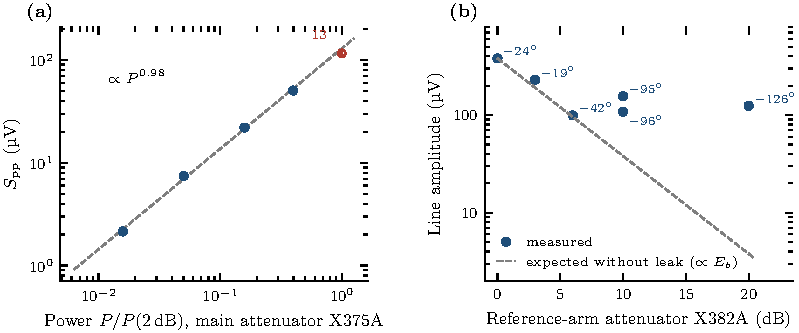
\includegraphics[width=\textwidth]{figures/power.pdf}
  \caption{Role of the two attenuators. The main attenuator X375A sits before the magic T and sets the microwave power
  at the cavity (and the reference with it). The reference-arm attenuator X382A only weakens the reference wave and
  leaves the power at the cavity unchanged. (a)~Power series with the main attenuator X375A (scans 24 to 27 at
  \qtyrange{6}{20}{dB}, scan 13 at \qty{2}{dB}):
  peak-to-peak signal versus power relative to \qty{2}{dB}; dashed: the fit to 24 to 27. Scan~13 (red)
  comes from an earlier measurement block. (b)~Series with the reference-arm attenuator X382A (scans 13 to 17b):
  magnitude of the line, $|a+\ii d|$ from \cref{eq:convolution}, and its phase $\arg(a+\ii d)$ (for the signal $S=-X$). Dashed: the decrease if the
  signal were proportional to the reference amplitude, which passes through X382A twice.}
  \label{fig:power}
\end{figure}

\paragraph{Power series.}
The main attenuator X375A sits before the magic T. It attenuates the wave to the cavity and the reference wave equally, so both amplitudes
grow with $\sqrt P$. By \cref{eq:diode} a square-law diode then gives a signal proportional to $E_bE_c\propto P$; a
detector measuring the amplitude instead of the power would give only $\sqrt P$. Over \qty{14}{dB} I find
$S_\mathrm{pp}\propto P^{\num{0.98(3)}}$ (\cref{fig:power}a). This is consistent with square-law detection, and I
found no sign of saturation over the investigated power range.

Saturation is not expected either. At most a few milliwatts reach the cavity, so the microwave field at the sample is
only $B_1\approx\qtyrange{3}{6}{\micro T}$. With $T_1\approx T_2=\qty{27}{ns}$ (plausible for an exchange-narrowed
radical) the saturation parameter $s=\gamma^2B_1^2T_1T_2$ is below \num{1e-3}; noticeable saturation would need more than
\qty{1}{W}. Scan~13 lies \qty{10}{\percent} below the straight line, but its line shape argues against saturation as well.
Saturation would reduce the absorption more than the dispersion. In scan~13 it is the other way round: the absorption
part is \qty{86}{\percent} of the mean of scans 24 to 27 (scatter \qty{8}{\percent}), the dispersion part only
\qty{52}{\percent} (scatter \qty{9}{\percent}). Since mainly dispersion is missing, I look for the cause in the bridge rather than in the spins (below).

\paragraph{Series with X382A.}
In scans 13 to 17b I changed the reference-arm attenuator X382A instead. It leaves the power at the cavity unchanged and only
weakens the reference wave $E_b$ in \cref{eq:diode}. The reference passes through it twice, so at \qty{20}{dB} $E_b$
drops by a factor of 100, and the signal $\propto E_b$ should drop by the same factor (dashed in \cref{fig:power}b).
In fact its magnitude drops only by a factor of 3.1, and its phase rotates by \ang{-102}, from mostly absorption to
mostly dispersion. I explain this with a \enquote{leak}: the cavity is not perfectly matched and itself sends a small
wave to the diode, of about a quarter of the reference amplitude. The weaker the reference, the more the leak takes over its role, and its
phase, not that of the plunger, decides which part of $\chi$ the diode sees. The signal is largest without attenuation
of the reference (\qty{0}{dB}). Only X375A is suitable for power series.

\paragraph{Size of the leak.}
I estimated the size of the leak from two independent measurements. With the leak $\rho e^{\ii\psi}$ added to the reference amplitude
$r=10^{-A/10}$ ($A$ is the X382A setting, passed twice), \cref{eq:diode} requires each part of the signal to be linear
in $r$. The absorption part is: $a=\alpha r+\beta$ with $\alpha=\qty{589}{\micro V}$ and $\beta=\qty{-73}{\micro V}$,
scatter \qty{6}{\micro V} for $r=\numrange{0.01}{0.5}$. The offset $\beta$ is the leak, and at $A=\qty{9.1}{dB}$ reference
and leak cancel in the absorption. The dispersion part is not reproducible. Scans 16 and 16b, taken with the same
settings, have the same absorption part (\qty{-12.3}{\micro V} and \qty{-12.0}{\micro V}) but dispersion parts of
\qty{-156}{\micro V} and \qty{-108}{\micro V}. The leak seems to drift, mainly in the dispersion, which is also the part
missing in scan~13.

The second measurement is the DC voltage of the diode at zero field, which I read on the oscilloscope for seven settings
of X382A between \qty{0}{dB} and \qty{20}{dB}. Without a line the diode sees only reference and leak,
$V_D=z-V_0\,|r+\rho e^{\ii\psi}|^2$, with the oscilloscope zero $z$ (the voltage is negative). The readings follow this
with $V_0=\qty{2.92(10)}{mV}$ and $\rho\cos\psi=\num{-0.204}$, scatter \qty{0.019}{mV}; for a single pass through X382A
the scatter would be five times larger. I did not measure $z$, but it must be at least the largest reading,
\qty{0.351}{mV}, so $\rho\geq\num{0.20}$. With $z=\qty{0.42}{mV}$, which also fits the line sizes of 13 to 17b,
$\rho=\num{0.26}$ and $\cos\psi=\num{-0.78}$. The leak is a quarter of the reference and partly cancels it: the diode
bias drops from \qty{1.93}{mV} at \qty{0}{dB} to \qty{0.08}{mV} at \qty{6.9}{dB}. Above about \qty{7}{dB} the leak is the
stronger wave, which is why the line turns into dispersion at \qtyrange{10}{20}{dB}.

The absorption part of scan~13 is also off the straight line (\qty{348}{\micro V} instead of \qty{516}{\micro V}).
Scaled to \qty{2}{dB}, scans 13 and 24 to 27 reach on average only 0.76 of the line value, as if \qty{1.2(4)}{dB} less
power had reached the cavity than in 14 to 18. At 15:53 I wrote in my lab notebook that I might have set X375A to
\qty{1}{dB} instead of \qty{2}{dB} before. Such a step between the blocks would explain the difference. I compare
signal sizes and phases only within one block; positions, widths and line shapes are not affected.

% --------------------------------------------------------------------
\subsection{Dispersion and guide wavelength}\label{sec:dispersion}

\begin{figure}[t]
  \centering
  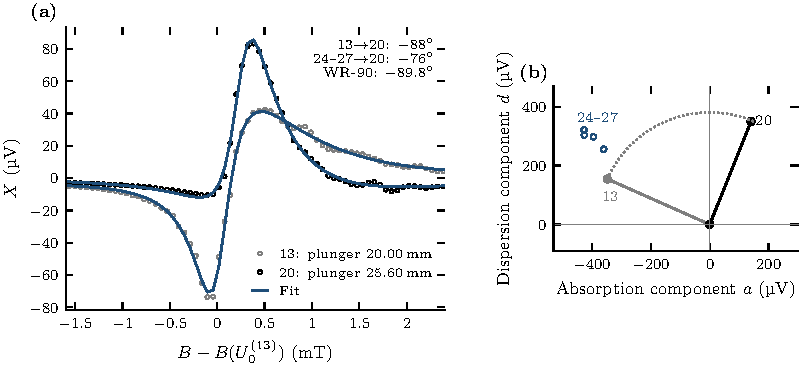
\includegraphics[width=\textwidth]{figures/dispersion.pdf}
  \caption{Dispersion. (a)~Scan~13 (plunger at \qty{20.00}{mm}) and scan~20 (\qty{25.60}{mm}), otherwise identical
  settings, shown as the signal $S=-X$, with fits according to \cref{eq:convolution}. The angles at the top right are the measured phase rotations and the
  value for WR-90. (b)~Complex amplitudes $a+\ii d$ of the lines: 13, 20 and 24 to 27 (same plunger position as 13,
  scaled to the same power); dotted: the rotation by the WR-90 value.}
  \label{fig:dispersion}
\end{figure}

For scan~20 I moved only the plunger, from \qty{20.00}{mm} (scan~13) to \qty{25.60}{mm}. This is
$\Delta z=\qty{5.60}{mm}$, almost exactly $\lamg/8$, i.e., $\lamg/4$ in the path of the reference wave (preparatory exercise~2). The line with a zero crossing at the center
becomes a line with a minimum at the center and two shallow side maxima (\cref{fig:dispersion}a): $\dd\chiII/\dd B$ turns
into $-\dd\chiI/\dd B$, as expected for a bridge phase rotated by \ang{-90} (\cref{eq:diode}).

To quantify this, I combine the absorption part $a$ and the dispersion part $d$ of each line (\cref{eq:convolution}) into the
complex amplitude $a+\ii d$. Its angle is the effective bridge phase $\varphi$ in \cref{eq:diode}: the phase of the
total reference wave at the diode, to which the leak from the cavity (\cref{sec:power}) contributes besides the
reference arm. The plunger rotates it by
\ang{-87.9} and leaves the magnitude unchanged (ratio \num{0.99}, \cref{fig:dispersion}b). Repeated scans at a fixed
plunger position scatter in phase by only \ang{1.1}, but the starting angle is uncertain. Scans 24 to 27, taken at the
same plunger position as 13 and shortly before scan~20, lie \ang{12} away from scan~13 because the leak drifts. With this
difference as a systematic uncertainty, $\Delta\varphi=\qty{-88(13)}{\degree}$, and $|\Delta\varphi|=4\pi\Delta z/\lamg$
together with \cref{eq:lamg_theory} gives
\begin{equation}\label{eq:lamg}
  \lamg=\frac{\ang{720}\,\Delta z}{|\Delta\varphi|}=46^{+8}_{-6}\,\unit{mm},\qquad
  \nu_\mathrm c=\nu\sqrt{1-(\lambda_0/\lamg)^2}=6.7^{+0.8}_{-1.1}\,\unit{GHz}.
\end{equation}
Despite the large uncertainty, the result is consistent with the WR-90 waveguide ($\lamg=\qty{44.9}{mm}$,
$\nu_\mathrm c=\qty{6.56}{GHz}$), and $\lamg$ is clearly larger than the free-space wavelength
$\lambda_0=\qty{32.0}{mm}$, which would correspond to \ang{-126}. The plunger displacement of \qty{5.60}{mm} also agrees
with the $\lamg/8$ needed to switch between absorption and dispersion.

\paragraph{Check without a line model.}
Absorption and dispersion are not independent. Because of causality (the spins cannot respond before they are driven),
$\chiI$ and $\chiII$ are Hilbert transforms of each other (Kramers--Kronig relations). The Hilbert transform $H$ commutes with the
derivative and with the smearing by the field distribution. The measured line $S_{13}$ and its transform $H[S_{13}]$ must
therefore give the line at any other bridge phase, whatever its exact shape:
\begin{equation}\label{eq:hilbert}
  S_{20}(U)=k\bigl[\cos D\,S_{13}+\sin D\,H[S_{13}]\bigr](U-\delta U)+b_0+b_1U .
\end{equation}
I computed $H[S_{13}]$ numerically from the data, with the fitted curve supplying the tails outside the scan window. The
fit gives $D=\qty{-84.3(7)}{\degree}$ and $k=\num{0.98}$. Its residuals (\qty{1.43}{\micro V}) are as small as those of
the free fit of scan~20 with \cref{eq:convolution} (\qty{1.41}{\micro V}). Within the noise, the two measured lines
therefore behave as a Kramers--Kronig pair, and the rotation angle follows without an assumption on the line shape. It
agrees with the \ang{-87.9} of the model fits within the systematic uncertainty. Starting from scans 24 to 26 instead of
13 gives \ang{-75} to \ang{-77}, an offset of about \ang{10}, like the one the drifting leak causes above.

% --------------------------------------------------------------------
\subsection{\texorpdfstring{\ce{MnCl2}}{MnCl2}: an exchange-narrowed line}\label{sec:mncl2}

\begin{figure}[t]
  \centering
  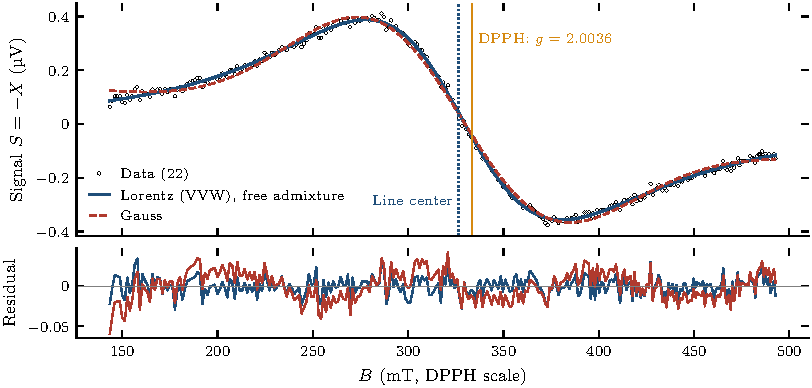
\includegraphics[width=\textwidth]{figures/mncl2.pdf}
  \caption{\ce{MnCl2}, scan~22 on the field scale with the reference \cref{eq:udmn}, shown as the signal $S=-X$. Blue: Lorentzian line according to
  \cref{eq:vvw} with free dispersion admixture and linear baseline; red dashed: Gaussian line. Bottom: the residuals.
  Vertical lines: line center (dotted) and the position that $g=\num{2.0036}$ would have at this frequency.}
  \label{fig:mncl2}
\end{figure}

\paragraph{Line shape and width.}
Scan~22 covers \qtyrange{143}{493}{mT} and shows a single line with $\Bpp\approx\qty{103}{mT}$ (\cref{fig:mncl2}); none
of the six hyperfine lines of \ce{^{55}Mn} is visible. The signal is small, \qty{0.74}{\micro V}, although \ce{MnCl2}
has a 76 times larger static susceptibility than DPPH, because the derivative of a line more than 400 times wider is
correspondingly flat. A Lorentzian describes the data within the noise (residuals \qty{1.5}{\percent} of the signal,
without visible structure). A Gaussian fits 1.6 times worse and misses the data on both flanks. A Lorentzian line is
what exchange narrowing predicts (\cref{sec:width}).

Because the line is so broad ($\Bhalf\approx0.27\,\Br$), a detail matters that plays no role for DPPH. Besides the
co-rotating component, the linearly polarized microwave field also has a counter-rotating one. It is resonant at
$B=-\Br$, and the tail of this second line reaches into the measurement window. The absorption is therefore
\begin{equation}\label{eq:vvw}
  \chiII(B)\propto\frac{1}{1+\Bigl(\frac{B-\Br}{\Bhalf}\Bigr)^2}+\frac{1}{1+\Bigl(\frac{B+\Br}{\Bhalf}\Bigr)^2}.
\end{equation}
Since the line is almost as wide as the measurement window, its position depends somewhat on the fit window and the
baseline: $g$ lies between \num{2.045} and \num{2.060}. Without the dispersion admixture I would get
$g=\numrange{2.028}{2.034}$, but that fit is clearly worse in every window I tried. The width is robust:
\begin{equation}\label{eq:mnwidth}
  \Bhalf=\qty{88.8(23)}{mT},\qquad T_2=\frac{1}{\gamma\Bhalf}=\qty{62(2)}{ps}.
\end{equation}
Without exchange, the dipolar fields of the neighbors would give a Gaussian line with an HWHM of about \qty{250}{mT}
(\cref{sec:width}). The measured line is a third as wide and Lorentzian. By \cref{eq:aw} this requires an exchange field
$B_\text{ex}\approx\qtyrange{0.5}{0.7}{T}$, comparable to the resonance field itself.

\paragraph{Field reference.}
For $g$, what matters is the field at which the scan passed the line center (\qty{4.854}{V}). The reference
$U_\text{D}$ from \cref{eq:fieldscale} does not apply, because scan~22 reached the line only after a run-up of
\qty{2.9}{V}, while the DPPH reference scans had a run-up of only \qty{38}{mV} (\cref{sec:field}). I take the
reference from the DPPH scans with a long run-up. Scans 07b and 08 (\qty{128}{mV} run-up) give \qty{4.9626}{V}, and the
DPPH search scan~06 (\qty{383}{mV}) gives \qty{4.983}{V}. They differ by only \qty{20}{mV} despite three times the
run-up, so the field lag stops growing after a few hundred millivolts. I assume that the reference of scan~22 lies
between these two values. Taking this bracket as a uniform distribution and adding the reading uncertainty and the drift
gives
\begin{equation}\label{eq:udmn}
  U_\text{D}^{(22)}=\qty{4.973(12)}{V}.
\end{equation}

\paragraph{\texorpdfstring{$g$}{g}-factor.}
Relative to this reference (\cref{eq:grel}),
\begin{equation}\label{eq:gmn}
  g\bigl(\text{\ce{MnCl2}}\bigr)=\num{2.058(11)} .
\end{equation}
The uncertainty comes mainly from the line shape (fit window and baseline, \num{0.008}), from the sample in the cavity
(\num{0.005}) and from the field reference (\num{0.005}). The sample detunes the cavity slightly, sees a field that is
not quite homogeneous, like DPPH, and shifts the field inside it with its own magnetization. Statistics, field scale and
$g_\text{DPPH}$ together contribute \num{0.003} (\cref{app:errors}). A gap in my lab notebook leaves a one-sided
systematic. Before scan~22 I set the field to \qty{5.9}{V} to adjust the lock-in phase, and I did not write down whether
I brought it back to \qty{0}{V} afterwards. If not, the scan ran on a different branch of the hysteresis curve, and $g$
would be smaller by up to \num{0.025}.

The line width lets me test this. On the other branch the field would rise more slowly across the line, because the gap
to the normal branch shrinks from \qty{5.6}{mT} at \qty{4.2}{V} to \qty{1.6}{mT} at \qty{5.6}{V} (estimated from the
hysteresis loop in \cref{fig:field}a). Scan~22 would then look 1.054 times wider than the search scan I recorded just
before, which did start from \qty{0}{V} (\qtyrange{2.00}{7.95}{V} at \qty{50}{mV/s}; signal in $Y$, because I set the
lock-in phase only afterwards). A joint fit of both scans, each part weighted by its own scatter, gives a width ratio of
\num{0.963(39)}. This is $2.3\sigma$ below the prediction for the other branch and $0.9\sigma$ below the normal branch.
The test favors the normal branch but cannot rule out the other one, on which $g=\num{2.032(11)}$.

\paragraph{Origin of \texorpdfstring{$g>2$}{g > 2}.}
For \ce{Mn^2+} without orbital moment one expects $g=\numrange{2.000}{2.002}$~\cite{abragam1970}; the measured value is
\num{0.057(11)} higher. I do not think this is an error of the field scale. A more likely explanation is the large width itself. The dipolar
coupling between the spins does not only broaden the line; it also contains terms that flip spins at the frequencies $\omega_0$
and $2\omega_0$. For narrow lines they average out, but for a line as wide as a quarter of the resonance field they shift
the resonance to higher frequency, that is, to lower field at fixed frequency, and $g$ appears larger. From the measured
width and without a free parameter, the theory of Kubo and Tomita~\cite{kubo1954} predicts $\Delta g=\numrange{0.028}{0.055}$,
which is consistent with the measurement.

% --------------------------------------------------------------------
\subsection{\texorpdfstring{\ce{Cu^2+}}{Cu2+}: no usable result}\label{sec:cu}
Scan~29 on the copper sample shows only noise (\qty{0.021}{\micro V}) and no line. This says nothing about \ce{Cu^2+},
however. In the repeat scan with the same settings the frequency counter showed \qty{9.199}{GHz}, about \qty{160}{MHz}
below the cavity resonance; when retuning I had not found a real dip. This far from resonance the signal is about 1000
times smaller. The noise of the scan still shows how sensitive it would have been on the dip: a single Lorentzian line
with $\Bpp=\qty{10}{mT}$ would have shown up ($3\sigma$) with only \qty{13}{\percent} of the number of spins in the DPPH
sample (\qty{3}{\percent} for \qty{5}{mT}, about as many as in DPPH for \qty{30}{mT}). The scan covered
$g=\numrange{1.89}{2.19}$. The measurement has to be repeated with a properly tuned source.
